\documentclass[12pt]{beamer}
\usepackage[utf8]{vietnam}
\usepackage{lmodern}
\usepackage{animate}
\usetheme{metropolis}
\begin{document}
	\author{Đặng Quang Anh - Nguyễn Trung Hiếu - Võ Huy Quang - Lê Thuý Quỳnh - Hoàng Minh Tuấn}
	\title{K-MEANS TRÊN MAPREDUCE}
	\date{Tháng 4 2021}
	%\subtitle{}
	%\logo{}
	%\institute{}
	%\date{}
	%\subject{}
	%\setbeamercovered{transparent}
	%\setbeamertemplate{navigation symbols}{}
	\maketitle
	\begin{abstract}
		K-Means là giải thuật phân cụm dữ liệu khá nổi tiếng và được sử dụng phổ biến trong lĩnh vực khai phá dữ liệu, nó cho phép chia $n$ đối tượng thành $k$ cụm sao cho tổng bình phương khoảng cách giữa các đối tượng đến tâm nhóm là nhỏ nhất. Tuy nhiên, phương pháp này còn nhiều hạn chế do việc tính khoảng cách giữa các đối tượng đến các tâm và xác định lại tâm được thực hiện lặp lại nhiều lần khiến giải thuật mất nhiều thời gian xử lí và khó triển khai trên tập dữ liệu lớn.\\
		Vì vậy chúng ta cần đến mô hình tính toán song song MapReduce để triển khai K-Means trên tập dữ liệu lớn.
	\end{abstract}

	\frame<beamer>{
		\frametitle{Outline}
		\tableofcontents
	}

	\section{Thuật toán phân cụm K-Means}
	\frame<beamer>{ 
		\tableofcontents[currentsection,currentsubsection] 
	}
	\begin{frame}
		\frametitle{Thuật toán phân cụm K-Means}
		\begin{enumerate} [\textbf{1.}]
			\item \textbf{Khái niệm giải thuật K-Means:}
					\begin{itemize}
						\item Là một thuật toán phân cụm đơn giản được sử dụng để giải quyết bài toán phân cụm
						\item Giải thuật gom cụm K-Means được sử dụng để phân loại tập dữ liệu phi cấu trúc hoặc bán cấu trúc, là 1 trong những phương thức phân loại dữ liệu phổ dụng và hiệu quả do tính đơn giản và khả năng kiểm soát tập dữ liệu
					\end{itemize}
		\end{enumerate}
	\end{frame}
	
	\begin{frame}
		\frametitle{Thuật toán phân cụm K-Means}
		\begin{enumerate} [\textbf{2.}]
			\item \textbf{Ứng dụng giải thuật K-Means:}
			\begin{itemize}
				\item Thuật toán K-Means thường được sử dụng trong các ứng dụng:
				\begin{itemize}
					\item Thống kê dữ liệu
					\item Công cụ tìm kiếm(Search engine)
					\item Phân loại khách hàng
				\end{itemize}
			\end{itemize}
		\end{enumerate}
	\end{frame}
	
	\begin{frame}
		\frametitle{Thuật toán phân cụm K-Means}
		\begin{enumerate} [\textbf{3.}]
			\item \textbf{Phương pháp giải thuật K-Means}
				\begin{itemize}
					\item \textbf{Bước 1:} Chọn k điểm bất kì trong tập dữ liệu làm tâm ban đầu.
					\item \textbf{Bước 2:} Với các điểm dữ liệu còn lại được gán cho cụm có khoảng cách đến tâm gần nhất.
					\item \textbf{Bước 3:} Tính toán lại khoảng cách để cho tâm cụm gần chính giữa cụm nhất
					\item Lặp lại bước 2 và 3 đến khi vị trí các tâm không đổi.
					\item[=>] \textbf{Nhược điểm:} Tiêu tốn tài nguyên hệ thống và thời gian, chỉ phù hợp với dữ liệu nhỏ và vừa.
				\end{itemize}
		\end{enumerate}
	\end{frame}

	\begin{frame}
		\frametitle{Thuật toán phân cụm K-Means}
		%chèn ảnh sơ đồ khối
		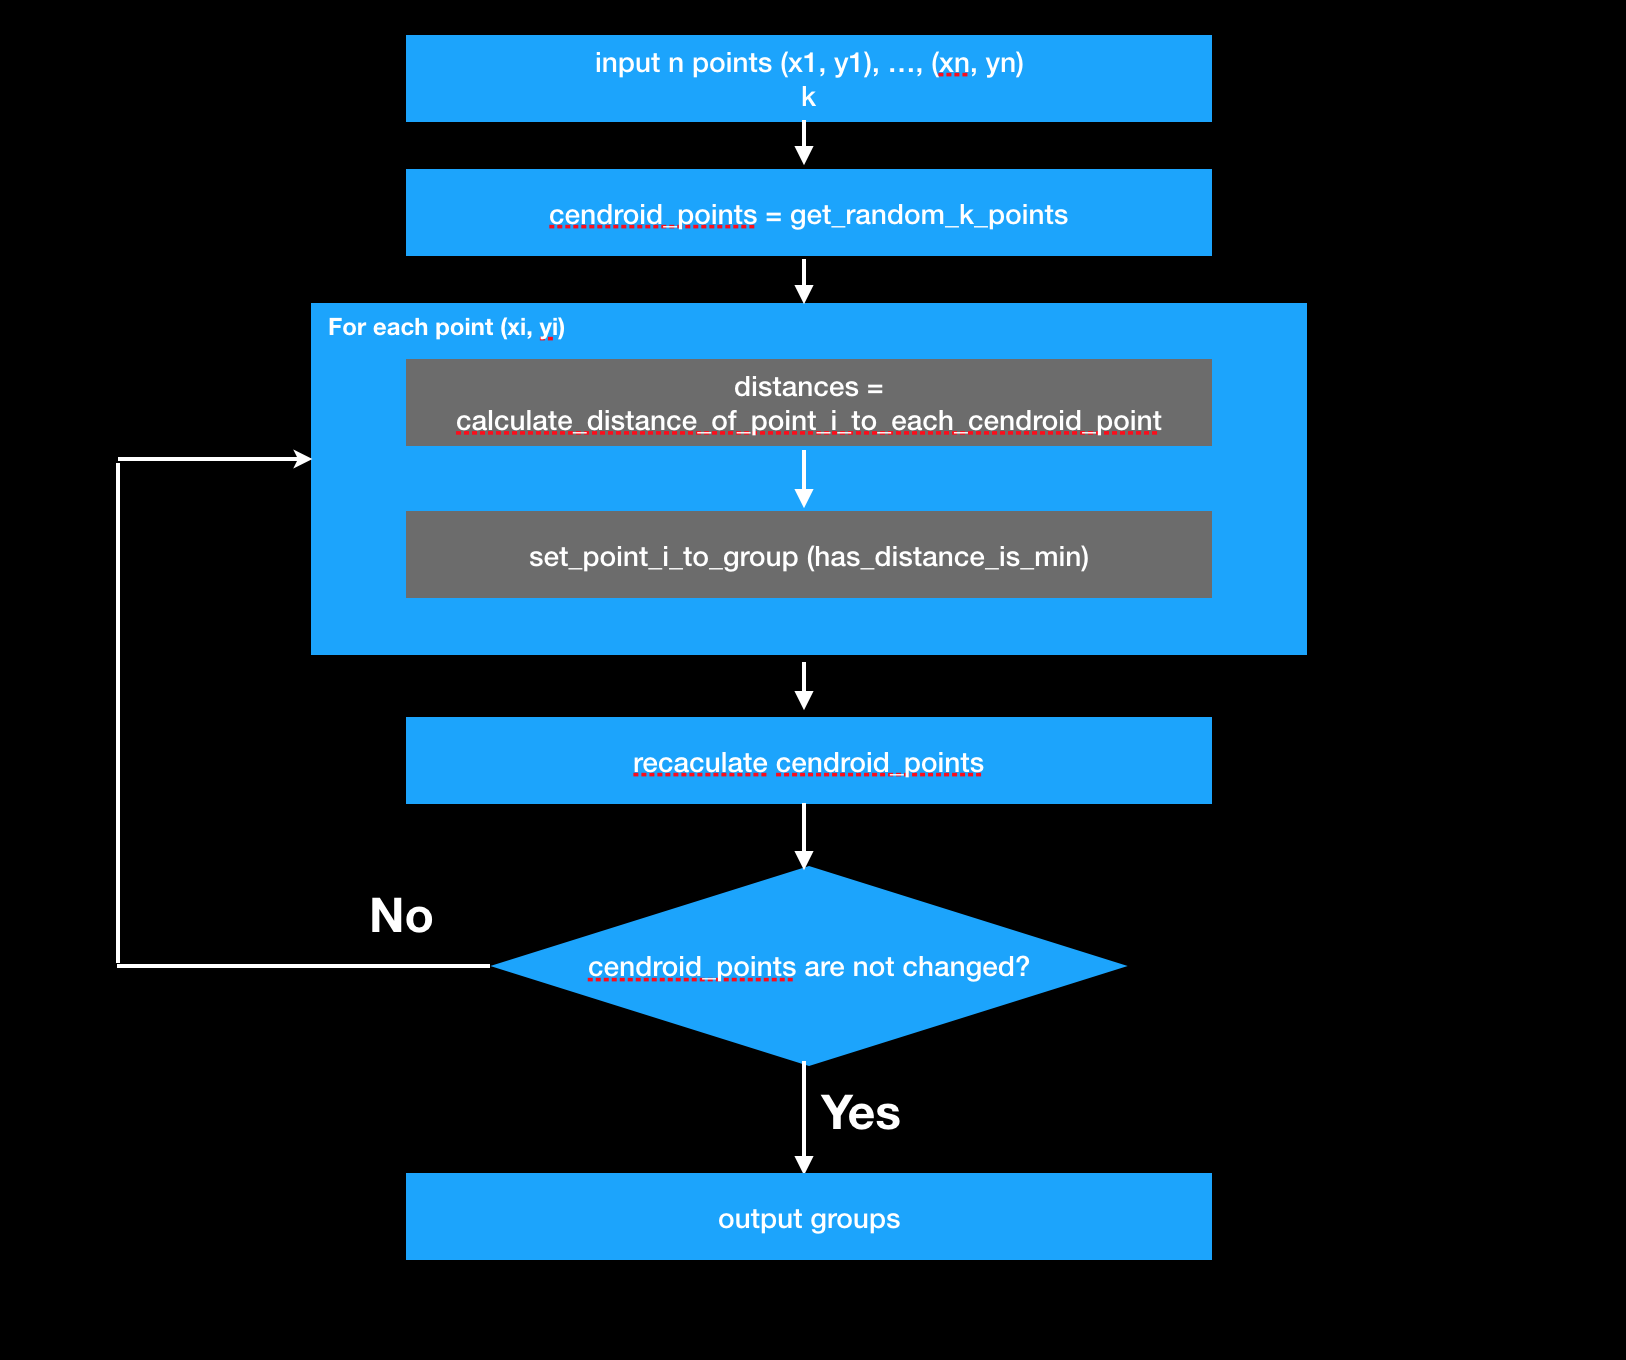
\includegraphics[scale=0.3]{kmean.png}
	\end{frame}

	\begin{frame}
		\frametitle{Thuật toán phân cụm K-Means}
		%chèn ảnh sơ đồ khối
		\animategraphics[controls, width=6cm]{1}{kmeans/kmeans-}{0}{13}
	\end{frame}
	
	\section{Mô hình MapReduce}
	\frame<beamer>{ 
		\tableofcontents[currentsection,currentsubsection] 
	}

	\begin{frame}
		\frametitle{Mô hình MapReduce}
		\begin{enumerate} [\textbf{1.}]
			\item \textbf{Khái niệm mô hình MapReduce}
				\begin{itemize}
					\item Là mô hình lập trình dùng để tính toán trên tập dữ liệu lớn
					\item Một trình xử lý MapReduce có thể tính toán đến terabytes hoặc petabytes dữ liệu trên hệ thống được kết nối thánh cụm các nodes.
					\item Ứng dụng:
						\begin{itemize}
							\item Thống kê số lượt truy cập URl.
							\item Thống kê số từ khoá trên các hotnames.
							\item ...
						\end{itemize}
					\item MapReduce gồm 2 pha: Map và Reduce.
				\end{itemize}
		\end{enumerate}
	\end{frame}

	\begin{frame}
		\frametitle{Mô hình MapReduce}
		%chèn ảnh sơ đò MapReduce
		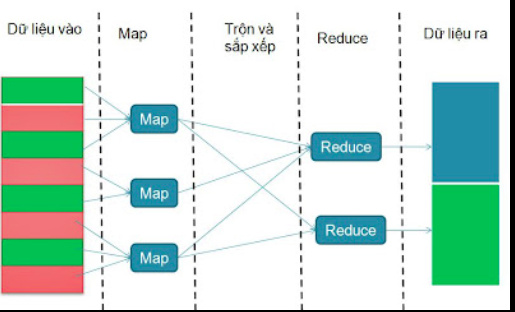
\includegraphics[width=\linewidth]{MapReduce.png}
	\end{frame}

	\begin{frame}
		\frametitle{Mô hình MapReduce}
		\begin{enumerate} [\textbf{2.}]
			\item \textbf{Bộ ánh xạ (Mapper):}
				\begin{itemize}
					\item Xử lý tập dữ liệu đầu vào dưới dạng $(key, value)$ và tạo lập trung gian là cặp $(key, value)$
					\item Bộ ánh xạ thực hiện 3 bước sau :
						\begin{itemize}
							\item Bước 1: Ánh xạ cho mỗi nhóm dữ liệu đầu vào dạng $(key, value)$
							\item Bước 2: Xử lý đầu vào -> chia nhóm -> tạo ra các $(key, value)$ trung gian.
							\item Bước 3: Đầu ra bộ ánh xạ được lưu trữ và định vị trong mỗi bộ Reducer.
						\end{itemize}
				\end{itemize}
		\end{enumerate}
	\end{frame}

	\begin{frame}
		\frametitle{Mô hình MapReduce}
		\begin{enumerate} [\textbf{3.}]
			\item \textbf{Bộ Reducer:}
			\begin{itemize}
				\item Trộn tất cả các phần tử có cùng $key$ trong tập dữ liệu tạo ra bởi Mapper để hình thành tập giá trị nhỏ hơn.
				\item Bộ Reducer thực hiện 3 bước sau :
				\begin{itemize}
					\item Bước 1: Đầu vào của Reducer là đầu ra của Mapper. MapReduce sẽ gắn khối liên quan cho bộ Reducer.
					\item Bước 2: Đầu vào của Reducer được gom theo $key$ -> giai đoạn trộn và sắp xếp.
					\item Bước 3: Tạo bộ so sánh để nhóm các $key$ trung gian lần 2 nếu quy luật gom nhóm khác với trước đó.
				\end{itemize}
			\end{itemize}
		\end{enumerate}
	\end{frame}

	\begin{frame}
		\frametitle{Mô hình MapReduce}
		\begin{enumerate} [\textbf{4.}]
			\item \textbf{Hoạt động của MapReduce}
				\begin{itemize}
					\item Đọc dữ liệu đầu vào.
					\item Xử lý dữ liệu đầu vào (Map).
					\item Sắp xếp và trộn các kết quả thu được từ các máy tính phân tán thích hợp.
					\item Tổng hợp các kết quả trung gian thu được (Reduce).
					\item Đưa ra kết quả cuối cùng.
				\end{itemize}
		\end{enumerate}
	\end{frame}
	
	\begin{frame}
		\frametitle{Mô hình MapReduce}
		%chèn ảnh sơ đồ MapReduce
		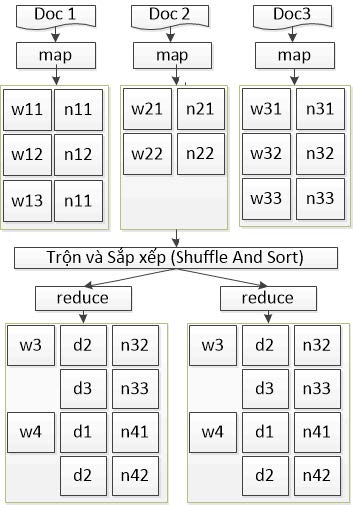
\includegraphics[scale=0.9]{MapReduce.jpg}
	\end{frame}
	
	\section{Thuật toán MRK-MEANS (MAPREDUCE K-MEANS)}
	\frame<beamer>{ 
		\tableofcontents[currentsection,currentsubsection] 
	}

	\begin{frame}
		\frametitle{Cách hoạt động của thuật toán MRK-MEANS}
		Thuật toán K-Means dựa trên mô hình MapReduce như sau:
		\begin{enumerate}[Bước 1:]
			\item Partition:\\
					Khởi tạo $k$ tâm ban đầu và chia tập dữ liệu thành các tập dữ liệu con nhỏ hơn
			\item Local clustering:\\
					Thực hiện tính toán để phân cụm trong từng bộ dữ liệu con\\
					\begin{itemize}
						\item Mapper: Đọc dữ liệu $x_i$ và tìm tâm $y_j$ gần với $x_i$ nhất.\\
								Tức là, $j = argmin_i || x_i - y_j ||_2$ và phát ra $<j, x_i>$
						\item Combiner: Lấy $<j, \left\{ x_i \right\}>$ và phát ra $<j, \Sigma x_i, num>$ trong đó $num$ là số đối tượng mà Combiner nhận khóa $j$
					\end{itemize}
		\end{enumerate}
	\end{frame}

	\begin{frame}
		\frametitle{Cách hoạt động của thuật toán MRK-MEANS}
		Thuật toán K-Means dựa trên mô hình MapReduce như sau:
		\begin{enumerate}[Bước 3:]
			\item Global clustering:\\
			Gộp cụm ở bộ dữ liệu lớn và tính toán lại tâm mới\\
			\begin{itemize}
				\item Reducer: Lấy $<j, \left\{ (\Sigma x_i, num) \right\}>$ và tính tâm mới, phát ra tâm mới $<j, y_j>$ của cụm
			\end{itemize}
		\end{enumerate}
		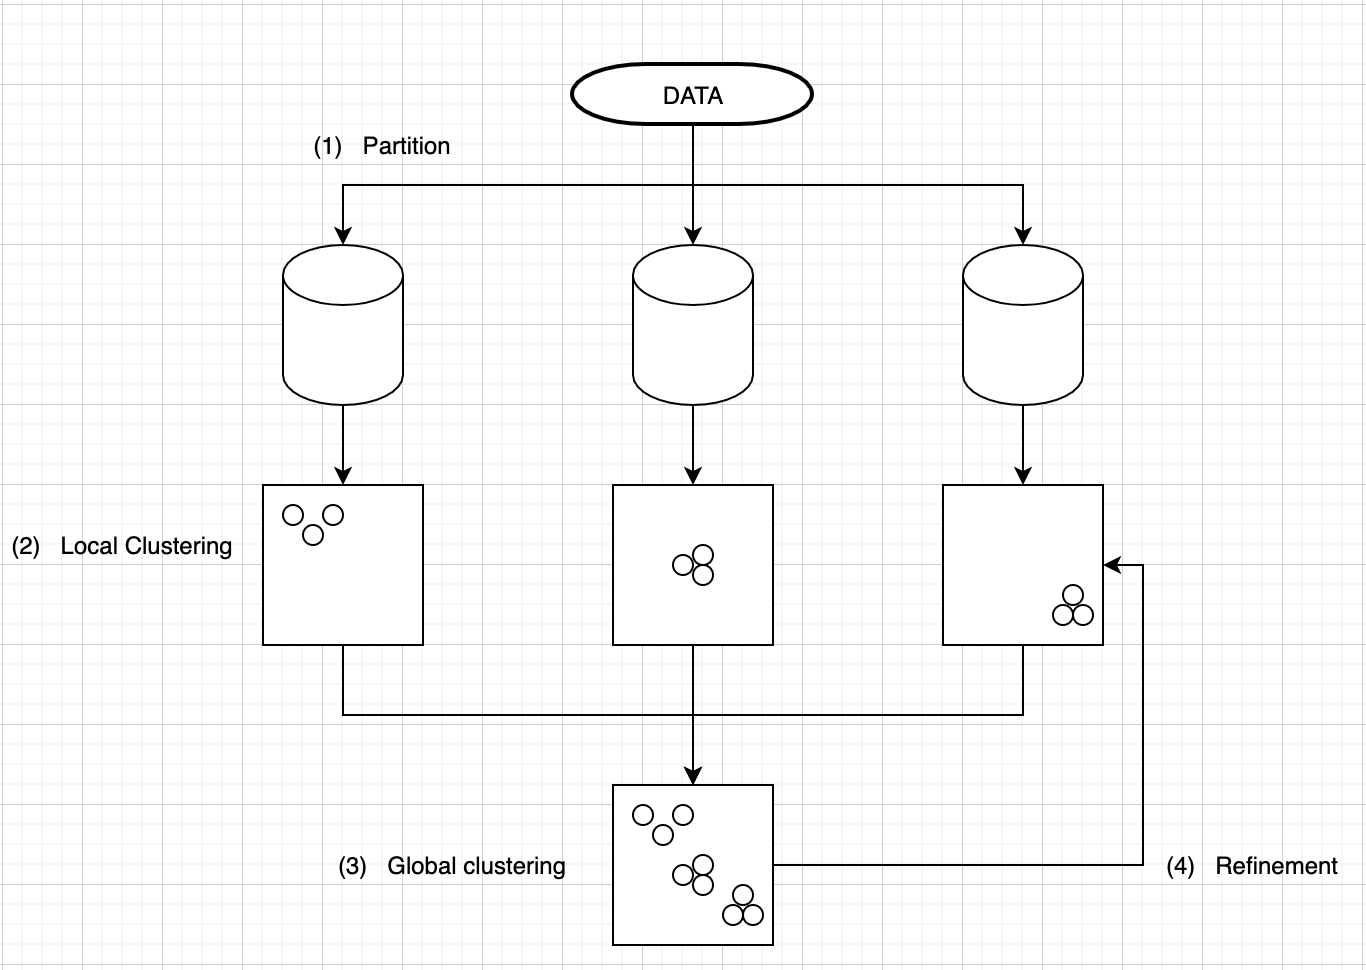
\includegraphics[scale=0.27]{MRK-Means.png}
	\end{frame}
	
\end{document}